\documentclass{bmcart}

%%%%%%%%%%%%%%%%%%%%%%%%%%%%%%%%%%%%%%%%%%%%%%
%%                                          %%
%% CARGA DE PAQUETES DE LATEX               %%
%%                                          %%
%%%%%%%%%%%%%%%%%%%%%%%%%%%%%%%%%%%%%%%%%%%%%%

%%% Load packages
\usepackage{amsthm,amsmath}
\usepackage{graphicx}
%\RequirePackage[numbers]{natbib}
\RequirePackage{hyperref}
\usepackage{float}
\usepackage[utf8]{inputenc} %unicode support
%\usepackage[applemac]{inputenc} %applemac support if unicode package fails
%\usepackage[latin1]{inputenc} %UNIX support if unicode package fails


%%%%%%%%%%%%%%%%%%%%%%%%%%%%%%%%%%%%%%%%%%%%%%
%%                                          %%
%% COMIENZO DEL DOCUMENTO                   %%
%%                                          %%
%%%%%%%%%%%%%%%%%%%%%%%%%%%%%%%%%%%%%%%%%%%%%%

\begin{document}

	\begin{frontmatter}
	
		\begin{fmbox}
			\dochead{Research}
			
			%%%%%%%%%%%%%%%%%%%%%%%%%%%%%%%%%%%%%%%%%%%%%%
			%% INTRODUCIR TITULO PROYECTO               %%
			%%%%%%%%%%%%%%%%%%%%%%%%%%%%%%%%%%%%%%%%%%%%%%
			
			\title{Reposicionamiento de fármacos en COVID-19}
			
			%%%%%%%%%%%%%%%%%%%%%%%%%%%%%%%%%%%%%%%%%%%%%%
			%% AUTORES. METER UNA ENTRADA AUTHOR        %%
			%% POR PERSONA                              %%
			%%%%%%%%%%%%%%%%%%%%%%%%%%%%%%%%%%%%%%%%%%%%%%
			
			\author[
			  addressref={aff1},                  
			  email={iresanjim@uma.es}
			]{\inits{I.S.J.}\fnm{Irene} \snm{Sánchez Jiménez }}
			\author[
			  addressref={aff1},
			  corref={aff1},
			  email={clarajimenez@uma.es}
			]{\inits{C.J.V}\fnm{Clara} \snm{Jiménez Valverde}}
			\author[
			  addressref={aff1},
			  email={patriciatr99@uma.es}
			]{\inits{P.T.R}\fnm{Patricia} \snm{Trujillo Rodríguez}}
			\author[
			  addressref={aff1},
			  email={\texttt{luci\_vm@uma.es}}
			]{\inits{L.V.M}\fnm{Lucía} \snm{Valverde Martínez}}
			
			%%%%%%%%%%%%%%%%%%%%%%%%%%%%%%%%%%%%%%%%%%%%%%
			%% AFILIACION. NO TOCAR                     %%
			%%%%%%%%%%%%%%%%%%%%%%%%%%%%%%%%%%%%%%%%%%%%%%
			
			\address[id=aff1]{%                           % unique id
			  \orgdiv{ETSI Informática},             % department, if any
			  \orgname{Universidad de Málaga},          % university, etc
			  \city{Málaga},                              % city
			  \cny{España}                                    % country
			}
		
		\end{fmbox}% comment this for two column layout
		
		\begin{abstractbox}
		
			\begin{abstract} % abstract
			En esta investigación, se busca encontrar fármacos ya existentes que puedan combatir la acción del virus SARS\_Cov-2. Debido a la alta tasa de contagio que tiene, nos urge encontrar tratamientos eficaces en poco tiempo. Aunque se han probado medicamentos útiles en casos de virus similares, para encontrar un tratamiento adecuado contra el SARS\_Cov-2 es esencial cambiar la aproximación reduccionista por una más centrada en el sistema. 
			Por ello, en este trabajo se propone usar las proteínas humanas descubiertas del interactoma funcional SARS-humano, junto a otras relacionadas, para encontrar fármacos ya existentes que afecten la acción del virus. Usando las bases de datos STRING y ChEMBL, obtenemos en el experimento fármacos potenciales, así como información sobre ellos, que se podrá usar en estudios posteriores.
			%%%%%%%%%%%%%%%%%%%%%%%%%%%%%%%%%%%%%%%%%%%%%%%
			%% RESUMEN BREVE DE NO MAS DE 100 PALABRAS   %%
			%%%%%%%%%%%%%%%%%%%%%%%%%%%%%%%%%%%%%%%%%%%%%%%	

			\end{abstract}
			
			%%%%%%%%%%%%%%%%%%%%%%%%%%%%%%%%%%%%%%%%%%%%%%
			%% PALABRAS CLAVE DEL PROYECTO              %%
			%%%%%%%%%%%%%%%%%%%%%%%%%%%%%%%%%%%%%%%%%%%%%%
			
			\begin{keyword}
			\kwd{COVID-19}
			\kwd{fármacos}
			\kwd{proteínas}
			\kwd{interactoma}
			\end{keyword}
		
		
		\end{abstractbox}
	
	\end{frontmatter}
	

	
	%%%%%%%%%%%%%%%%%%%%%%%%%%%%%%%%%
	%% COMIENZO DEL DOCUMENTO REAL %%
	%%%%%%%%%%%%%%%%%%%%%%%%%%%%%%%%%
	
	\section{Introducción}
%\cite{Shulla2011}
A día de hoy, puede que la enfermedad más mencionada en todo el mundo sea el SARS-CoV-2 (coronavirus 2 del síndrome respiratorio agudo severo). Este virus, que se originó en la ciudad China de Wuhan en diciembre de 2019, se ha extendido a todos los países del mundo rápidamente. Aunque la tasa de mortalidad del 2\% no es especialmente alta, el SARS-CoV-2 es altamente contagioso y transmisible de persona en persona con un período de incubación de hasta 24 días \cite{Yan2020}. Este brote de SARS-CoV2 ha provocado grades impactos en la salud social y la economía en todos los niveles, convirtiéndo en una prioridad encontrar tratamientos eficientes para la enfermedad. 

Como podemos ver en la revisión bibliográfica \cite{Yan2020}, ya en los primeros 75 días del brote de COVID-19 se propusieron algunos tratamientos médicos para combatir el SARS-CoV-2. Los más usados fueron antivirales (oseltamivir, ganciclovir y KALETRA), agentes antibióticos (cefalosporina, quinolona y carbapenem) para prevenir infecciones secundarias, y en los casos más graves terapia de oxígeno y terapia de reemplazo renal. El uso de estos tratamientos se debe en su mayoría a la eficacia que han tenido en virus similares como es la influenza. 

Para maximizar la eficacia de los tratamientos empleados, es vital diseñar fármacos que ataquen al virus de forma directa. Sin embargo, esto supone dos inconvenientes. El primero es conocer una forma eficaz de combatir la enfermedad y el segundo es el largo proceso que conlleva diseñar un fármaco. 

Encontramos numerosos artículos que tratan de desentrañar el interactoma SARS-humano (\cite{Hoffmann2020}, \cite{Yan2020a}, \cite{Shulla2011}, \cite{Chan2020}, \cite{Gysi2020}). Conociendo las proteínas humanas que son afectadas por el virus, podemos encontrar fármacos que perjudiquen la acción de éste en los seres humanos. 

Debido a la urgencia de encontrar tratamientos efectivos, en nuestra investigación se propone encontrar fármacos ya existentes que actúen sobre las proteínas del interactoma entre SARS y humanos. 

Para hacer esta búsqueda, usaremos la base de datos ChEMBL. ChEMBL es un conjunto de datos 'quimogenómicos' que une información sintética, de bioactividad y genómica de medicamentos. Surgió ante la necesidad de indexar productos genéticos y conectarlos con medicamentos para su posterior análisis y divulgación por parte de farmacéuticas, pequeñas organizaciones y establecimientos académicos. 

En nuestro caso, ChEMBL nos permitirá obtener fármacos cuyas dianas sean proteínas humanas del interactoma SARS-Humano.

\newpage
	\section{Materiales y métodos}

Partimos nuestra investigación buscando el interactoma funcional SARS-humano. Aunque el SARS-CoV-2 es un virus reciente, encontramos en la literatura científica numerosos papers que investigan este tema ((\cite{Hoffmann2020}, \cite{Yan2020a}, \cite{Shulla2011}, \cite{Chan2020}, \cite{Gysi2020})). Como podemos ver en \cite{Gysi2020}), el genoma viral del SARS-CoV-2 es capaz de crear 29 proteínas diferentes. En el trabajo \cite{Shulla2011}, Gordon et aI. consiguieron aislar 27 de estas proteínas para estudiar aquellas proteínas humanas que interaccionan con las del SARS-CoV-2. Esta investigación encontró interacciones de proteínas humanas con 26 de las proteínas del SARS-CoV-2. 

Las proteínas humanas que pertenecen al interactoma funcional SARS-humano pueden ser la clave para frenar al virus, impidiendo que éste infecte a las células, se replique y se expanda. Sin embargo, diseñar fármacos específicos para el SARS-CoV-2 puede llevar mucho tiempo, por lo que vamos a estudiar qué fármacos existen actualmente cuya diana sean estas proteínas humanas. 

\subsection{STRING, base de datos de interacción de proteínas}

Como se habla en \cite{Chan2020}, cuando usamos fármacos con dianas específicas, podemos encontrar efectos en proteínas relacionadas. Esta idea se enmarca dentro de la corriente holística, donde debemos estudiar el sistema como un conjunto, en vez de centrarnos en las partes. 

Siguiendo esta reflexión, buscar proteínas que se relacionen directamente con nuestras proteínas diana, que llamaremos proteínas secundarias, y hallar fármacos que actúen sobre estas proteínas secundarias, puede llevarnos a tener tratamientos que indirectamente combatan la acción del virus. 

Para encontrar estas proteínas secundarias, vamos a hacer uso de STRING. STRING es una base de datos de interacciones de proteínas. Introducimos en STRING las proteínas humanas del interactoma SARS-humano que conocemos (un total de 332 proteínas) y hacemos un filtrado de la búsqueda. 

Primero, seleccionamos que la puntuación de la interacción (interaction score) sea de al menos 0.700, lo que nos asegura interacciones de alta confianza. A continuación, pedimos que se nos muestren hasta 100 proteínas que interaccionan con cada una de las introducidas. De esta forma, encontramos las proteínas secundarias para nuestro estudio. 

    \subsubsection{Mapeo de códigos}
    Tras hacer nuestra búsqueda en STRING, tenemos un listado de genes que codifican proteínas del interactoma SARS-Humano (332 genes) y otro listado que corresponde a los genes que codifica a las proteínas secundarias (115 genes).
    
    A continuación, debemos preparar estos datos para nuestro flujo, que requiere que los nombres de los genes se mapeen con el ID de CHEMBL. Este proceso lo hemos hecho usando la herramienta de mapeo Retrieve/ID que proporciona Uniprot. Sin embargo, durante el mapeo, el número de genes disminuye mucho, teniendo finalmente 88 proteínas del interactoma y 30 proteínas secundarias.

\subsection{Código desarrollado}

Para poder obtener los datos de CHEMBL hemos encontrado una serie de paquetes tanto en R como en Python que contienen las funciones deseadas.

\subsubsection{Trabajo en Python}
El principal paquete que existe y tiene acceso a CHEMBL es un cliente web que trabaja a través del lenguaje Python. Su nombre es \textbf{\textit{chembl\_webresource\_client}}, y CHEMBL tiene una sección web dedicada a explicar su funcionamiento. %PONER REFERENCIA

Al usar este paquete se nos presentan dos problemas. El primero es que los datos que obtenemos desde este servicio web no están conectados entre sí de la misma manera en que lo están los datos dentro de CHEMBL. Por tanto, acceder a un medicamento a partir de los targets (proteínas) disponibles no es algo fácil de hacer. El segundo problema se presenta una vez averiguamos cómo hacer esto, y es que los datos descargados no son siempre correctos, y en algunos casos una misma petición devuelve respuestas diferentes en cada ejecución. Esto nos hizo llegar a la conclusión de que no podíamos hacer un programa fiable con este paquete, y por tanto pasamos a otras opciones.

\subsubsection{Trabajo en R}
El paquete que tenemos disponible en R es muy básico, se llama \textbf{\textit{chemblr}} y fue modificado por última vez hace siete años, por lo que no está demasiado actualizado. %PONER REFERENCIA

En vez de basarnos en este paquete, vamos a obtener nuestra información a partir de peticiones GET a la web de CHEMBL. Usaremos de nuevo la página en la que se explica el funcionamiento del servicio web de python, solo que aplicaremos sus ejemplos sobre R. Para hacer esto, nos hemos ayudado de una página de la web de EMBL.  %REFERENCIAS

El paquete \textbf{\textit{chemblr}} lo usaremos simplemente para obtener los json en un formato cómodo. Todos los paquetes requeridos se instalarán en la carpeta \textit{software/deps} dentro de \textit{code}.

\subsubsection{setup.sh}
Para la carga de los distintos paquetes que vamos a usar durante el desarrollo de la actividad, utilizaremos la ventana de comandos. 

Hemos diseñado un script de bash llamado \textbf{\textit{setup.sh}}. En este script, creamos en primer lugar un repositorio local \textbf{deps} que deberá crearse dentro de la carpeta \textbf{software}. 

Antes de proceder a la carga de todas las librerías dentro de este repositorio, concedemos permisos de administrador a la misma. 

Hemos definido dos listas de paquetes, una para aquellos que se obtienen desde CRAN (jsonlite, httr, devtools, sjmisc, tidyverse, networkD3, magrittry) y  otra para aquellos que se obtienen a través del paquete previamente instalado devtools, que en nuestro caso es solo una (chemblr). 

Para cada una de estas listas, ejecutamos un bucle for dentro del cual se instalarán las librerías una por una. 

\subsubsection{launch.sh}
Para ejecutar todo el flujo de trabajo que hemos generado, utilizamos el archivo \textbf{\textit{setup.sh}}. A este archivo le pasamos como argumento un número, que puede ser \textbf{1}, \textbf{2}, \textbf{3} o \textbf{4}. Si le pasamos \textbf{1}, trabajaremos con fármacos en fase 3 y proteínas de primer grado de interacción; en el caso de pasar un \textbf{2}, utilizaremos fármacos en fase 3 y proteínas secundarias; de la misma manera ocurre con el \textbf{3} y el \textbf{4}, a diferencia de que en este caso los fármacos serán de fase 4. 

Este archivo primero cargará todas las librerías que hemos descargado previamente con \textbf{setup.sh} y estarán en la carpeta \textbf{deps} dentro de \textbf{software}. 

Posteriormente, se establecen las variables locales que vamos a usar durante el estudio. Seguidamente se cargan las funciones realizadas y se pasa a la ejecución, donde se utilizan esas funciones. 

Finalmente, se procede a guardar los archivos \textbf{CSV} y las gráficas que hayamos generado durante la actividad en la carpeta \textbf{results}. 


Aquí podemos ver cómo quedaría el flujo: 

\begin{figure}[h!]
			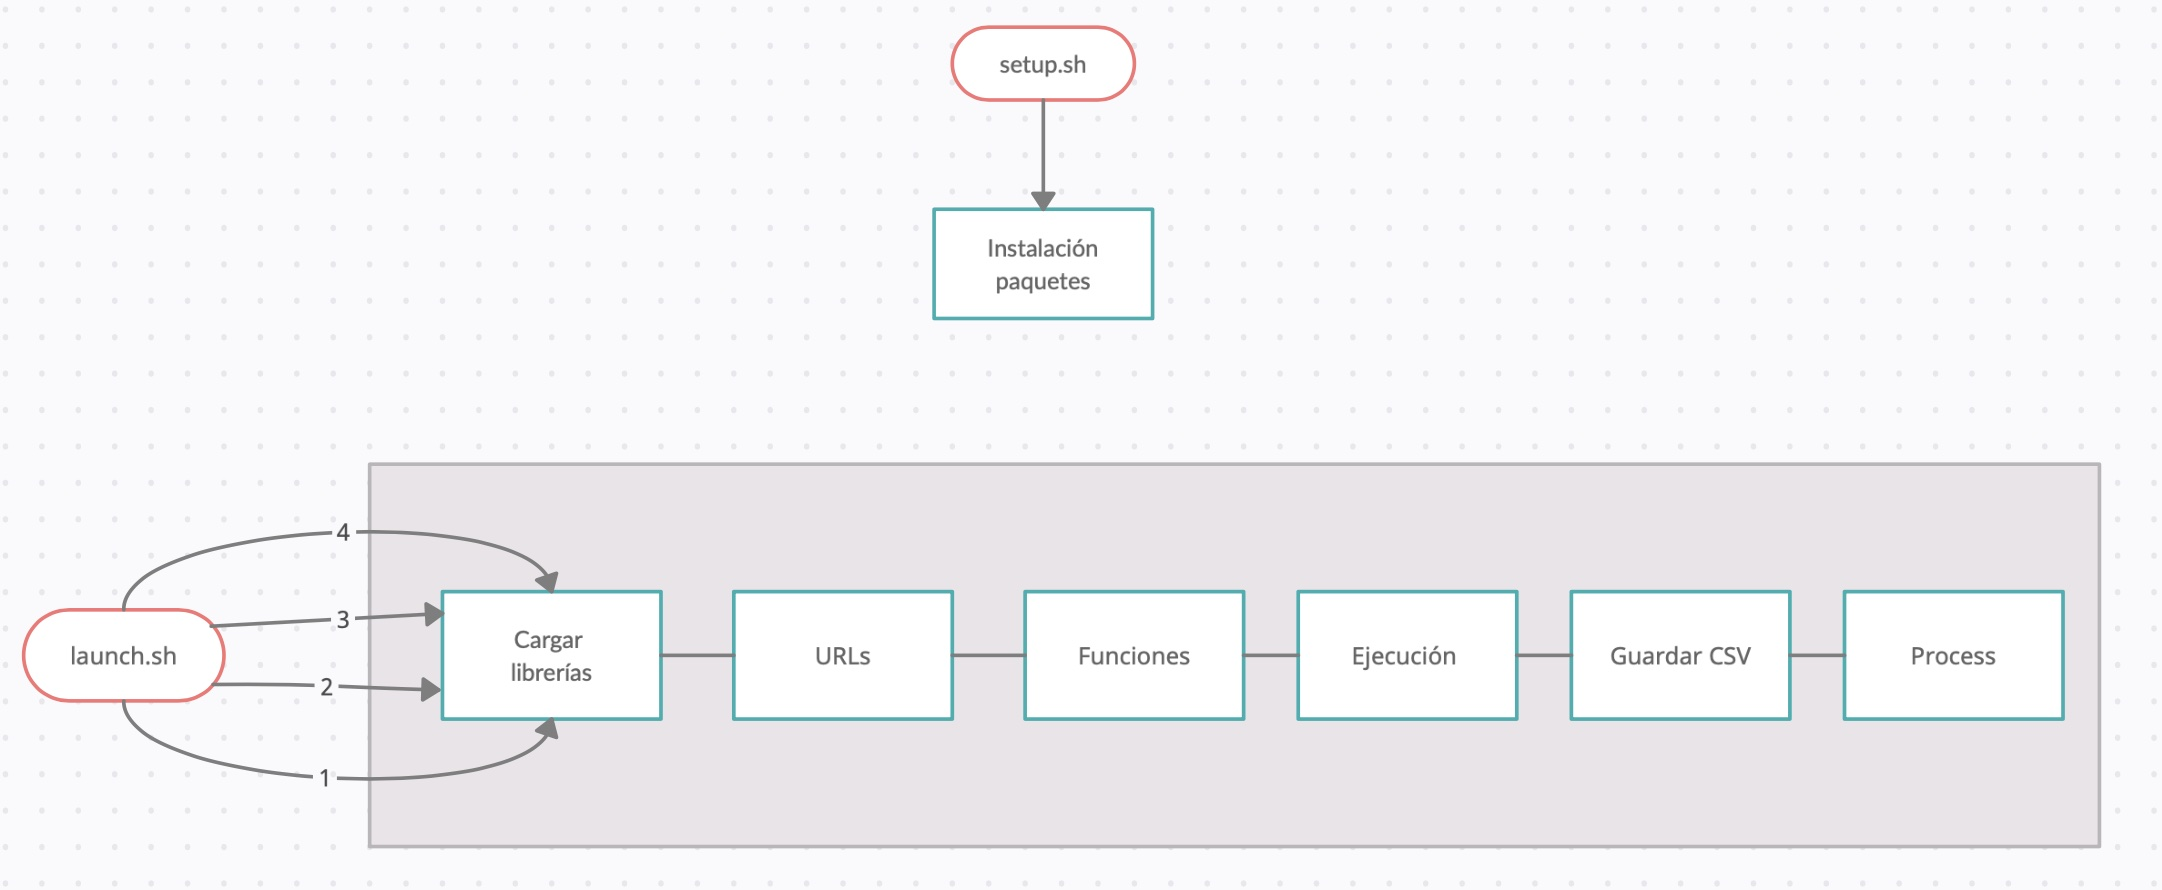
\includegraphics[width=0.9\textwidth]{figures/flujo.jpg}
			\caption{Flujo de trabajo}
		\end{figure}

\newpage
	\section{Resultados}
\subsection{Información de los fármacos}

Tras la ejecución de nuestro flujo de bash con sus cuatro opciones, en la carpeta de resultados vamos a tener un directorio para cada combinación de fase del ensayo clínco y del conjunto de proteínas diana buscadas. En la carpeta encontramos dos archivos csv, uno contiene información genérica del fármaco (id de ChEMBL del fármaco y de la proteína objetivo, fecha de aprobación, etc.) y el otro corresponde a la información química de cada fármaco encontrado. 

En nuestro trabajo, no usamos la información química obtenida para analizar los fármacos resultates de nuestra búsqueda. Sin embargo, como vemos en \cite{Poleto2018} datos químicos como el número de anillos aromáticos pueden ser de gran ayuda a la hora de estudiar los efectos de un fármaco sobre el organismo. Por ello, guardamos esta información y definimos en el anexo el significado de cada variable de los archivos csv.


\subsection{Gráficas en R}
Tras obtener los datos de los fármacos para fase del ensayo clínico 3 y 4 y para proteínas del interactoma SARS-Humano y las proteínas secundarias, vamos a realizar una serie de gráficos que nos ayuden a analizarlos. A continuación, mostraremos solo aquellos correspondientes a los fármacos de fase cuatro debido a que los de fase tres nos porporcionan muy pocos resultados. 

Lo primero que creamos es una gráfica de barras en la que representamos la frecuencia de cada tipo de acción tanto para las proteínas de primer grado como para las de segundo. Con esto buscamos obtener unda idea de cuál es más viable para ser utilizado contra el COVID-19. Estos tipos de acción se refieren a la manera en la que el fármaco interactúa con la proteína o con su entorno.

\begin{figure}[h]
			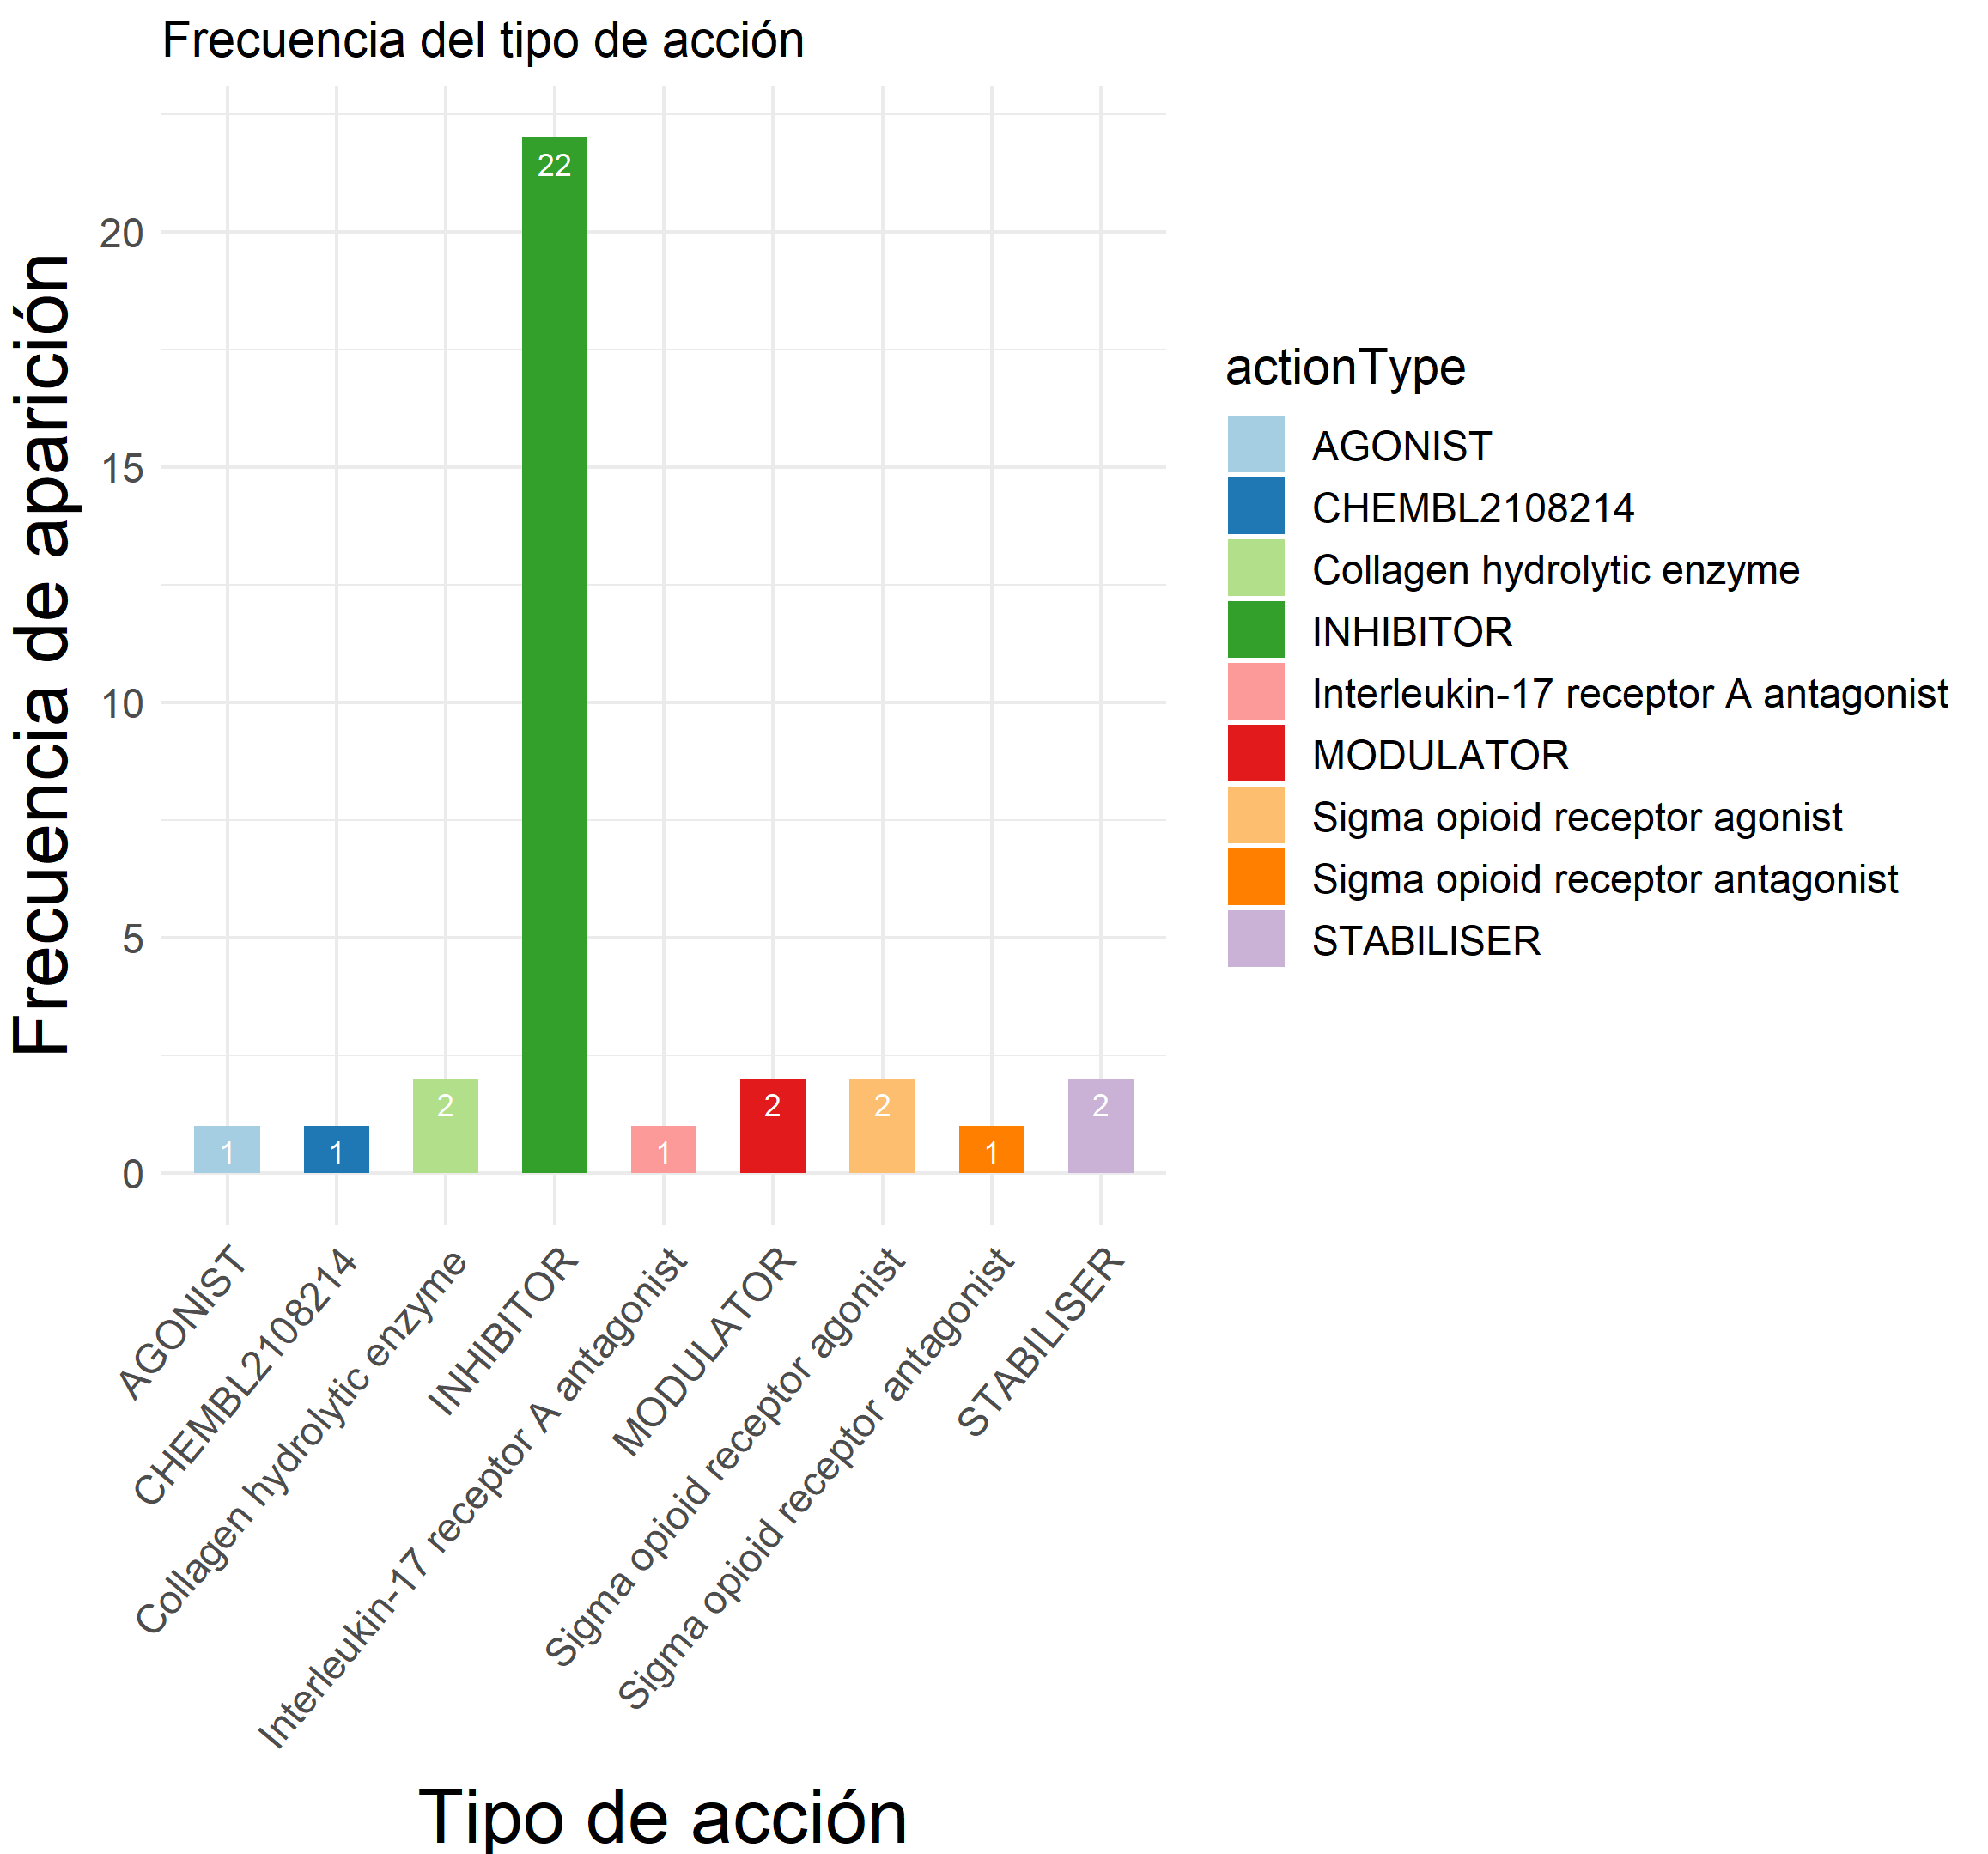
\includegraphics[width=0.9\textwidth]{figures/graficaTipoDeAccionProteinas1.png}
			\caption{Tipo de Acción, Proteínas de primer grado}
\end{figure}
\clearpage
\begin{figure}[h]
			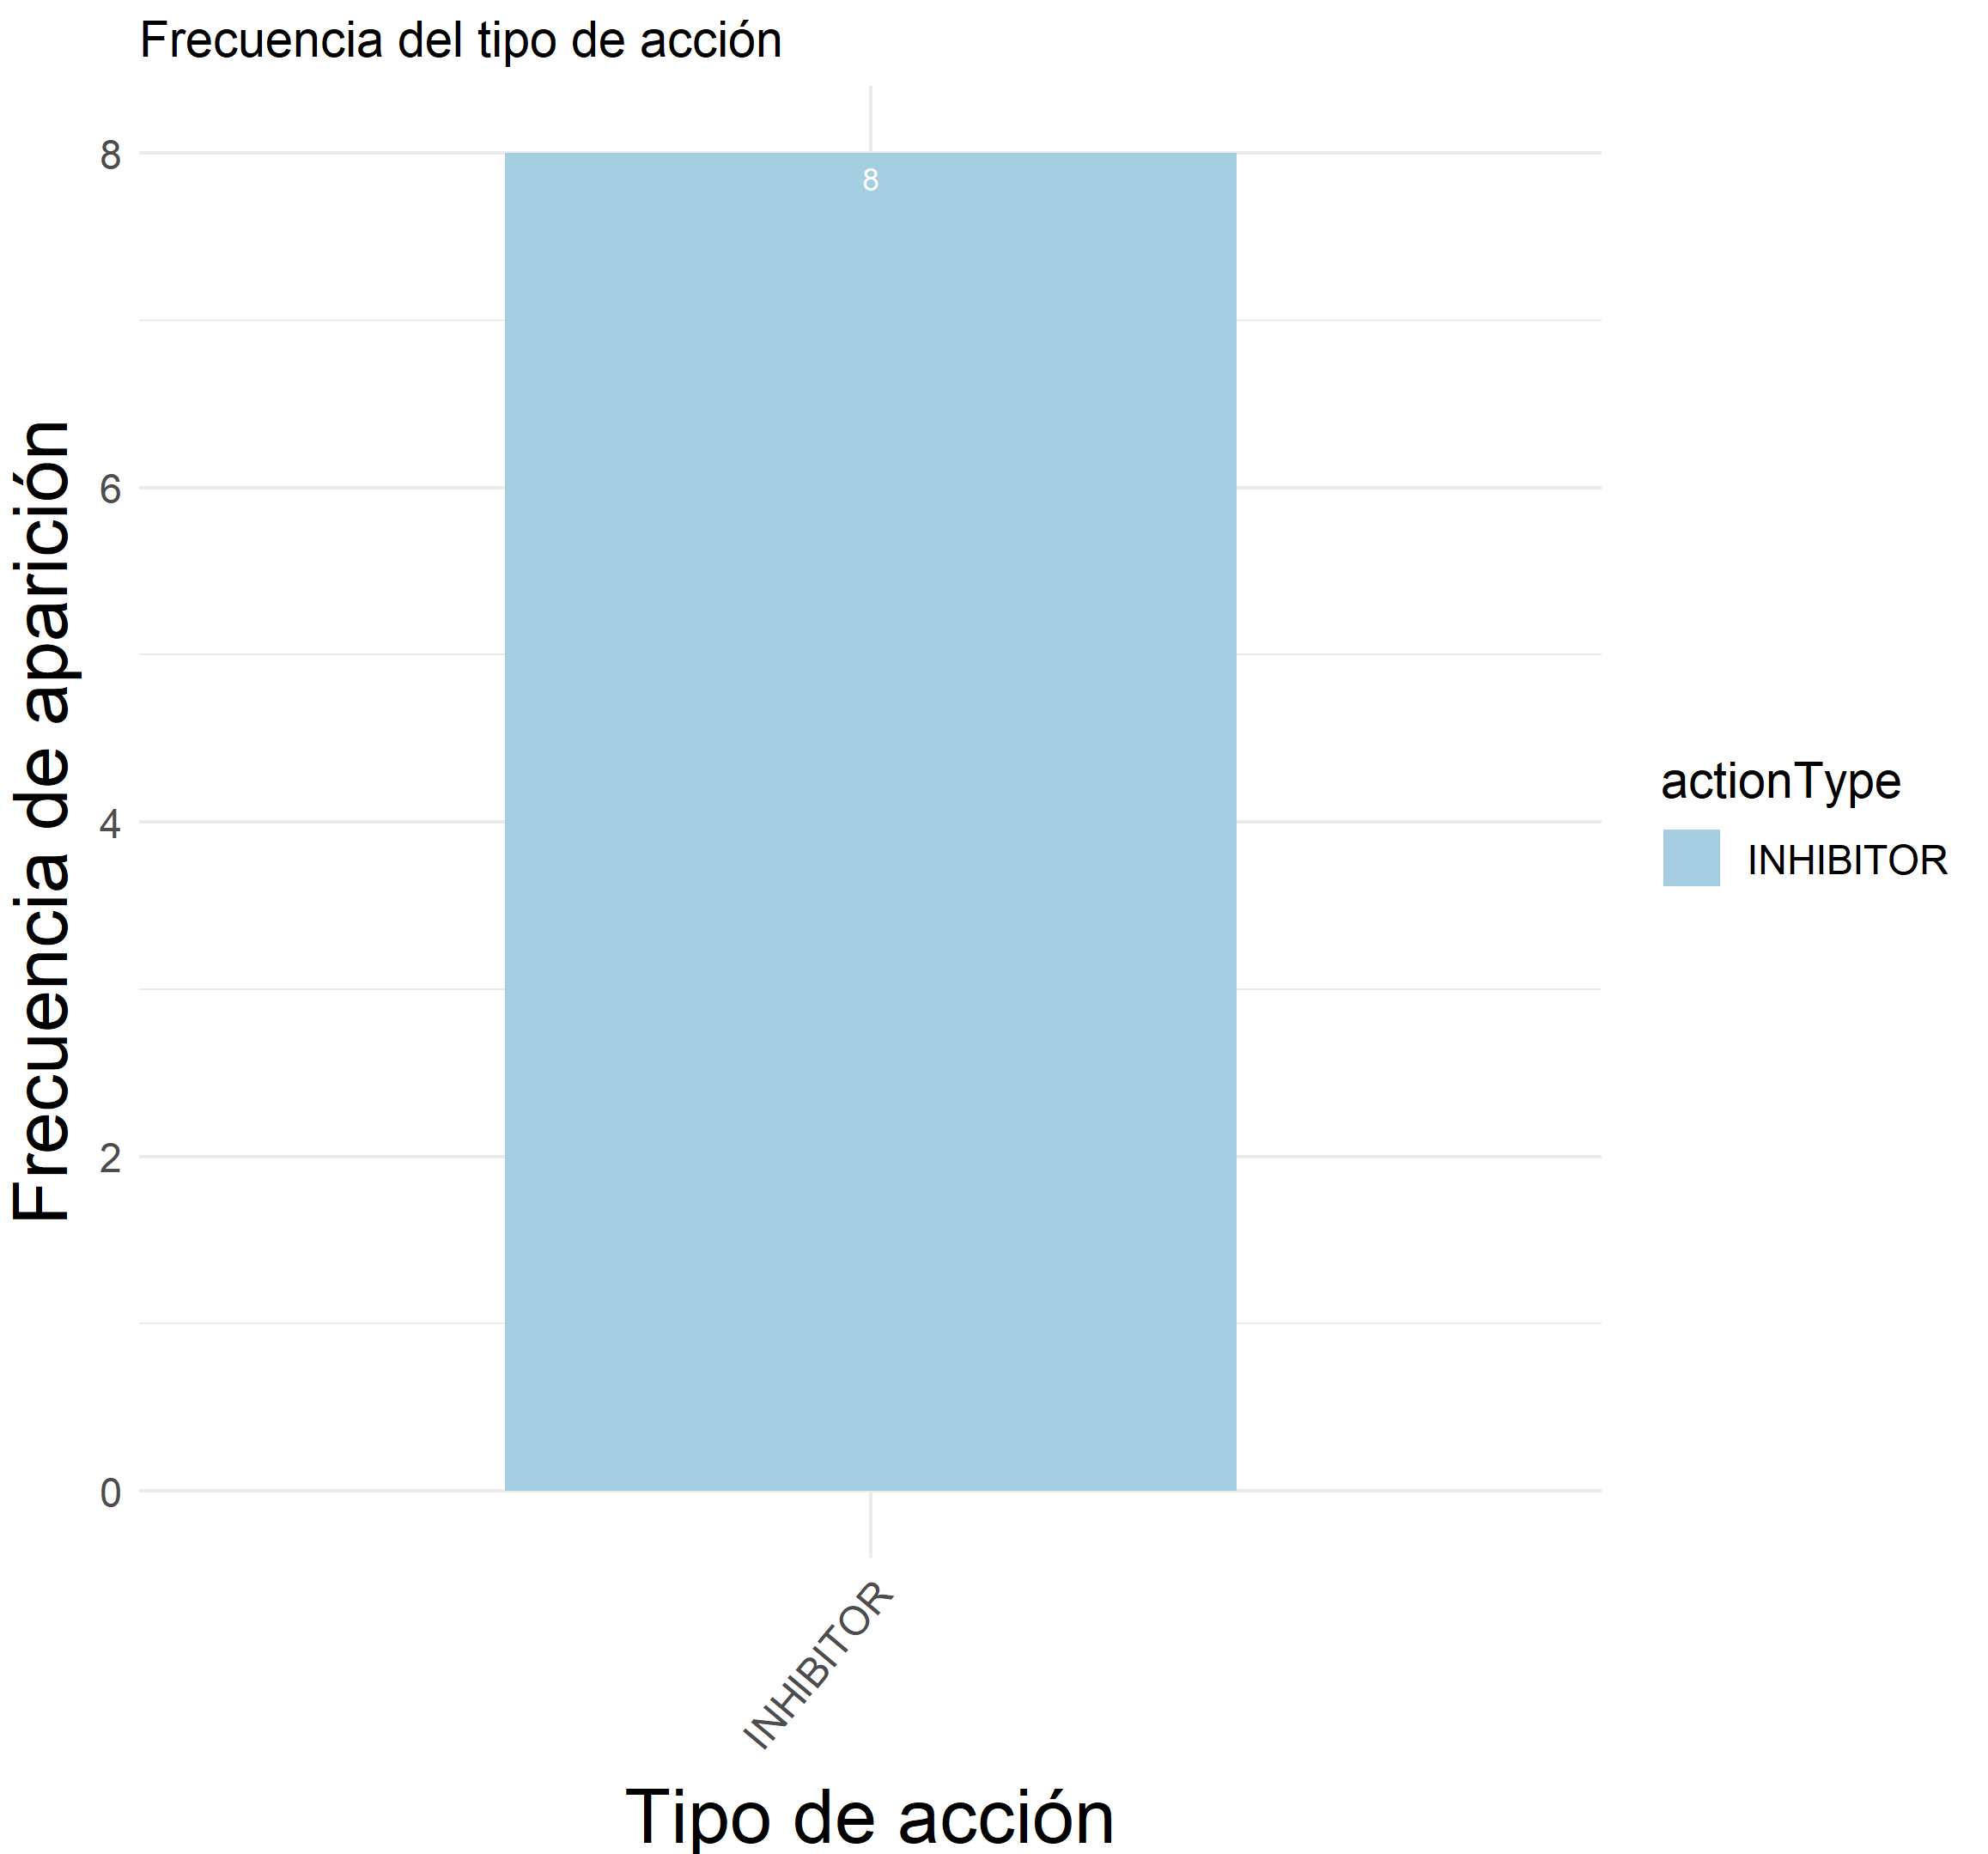
\includegraphics[width=0.9\textwidth]{figures/graficaTipoDeAccion.png}
			\caption{Tipo de Acción, Proteínas de segundo grado}
\end{figure}
%\clearpage 
%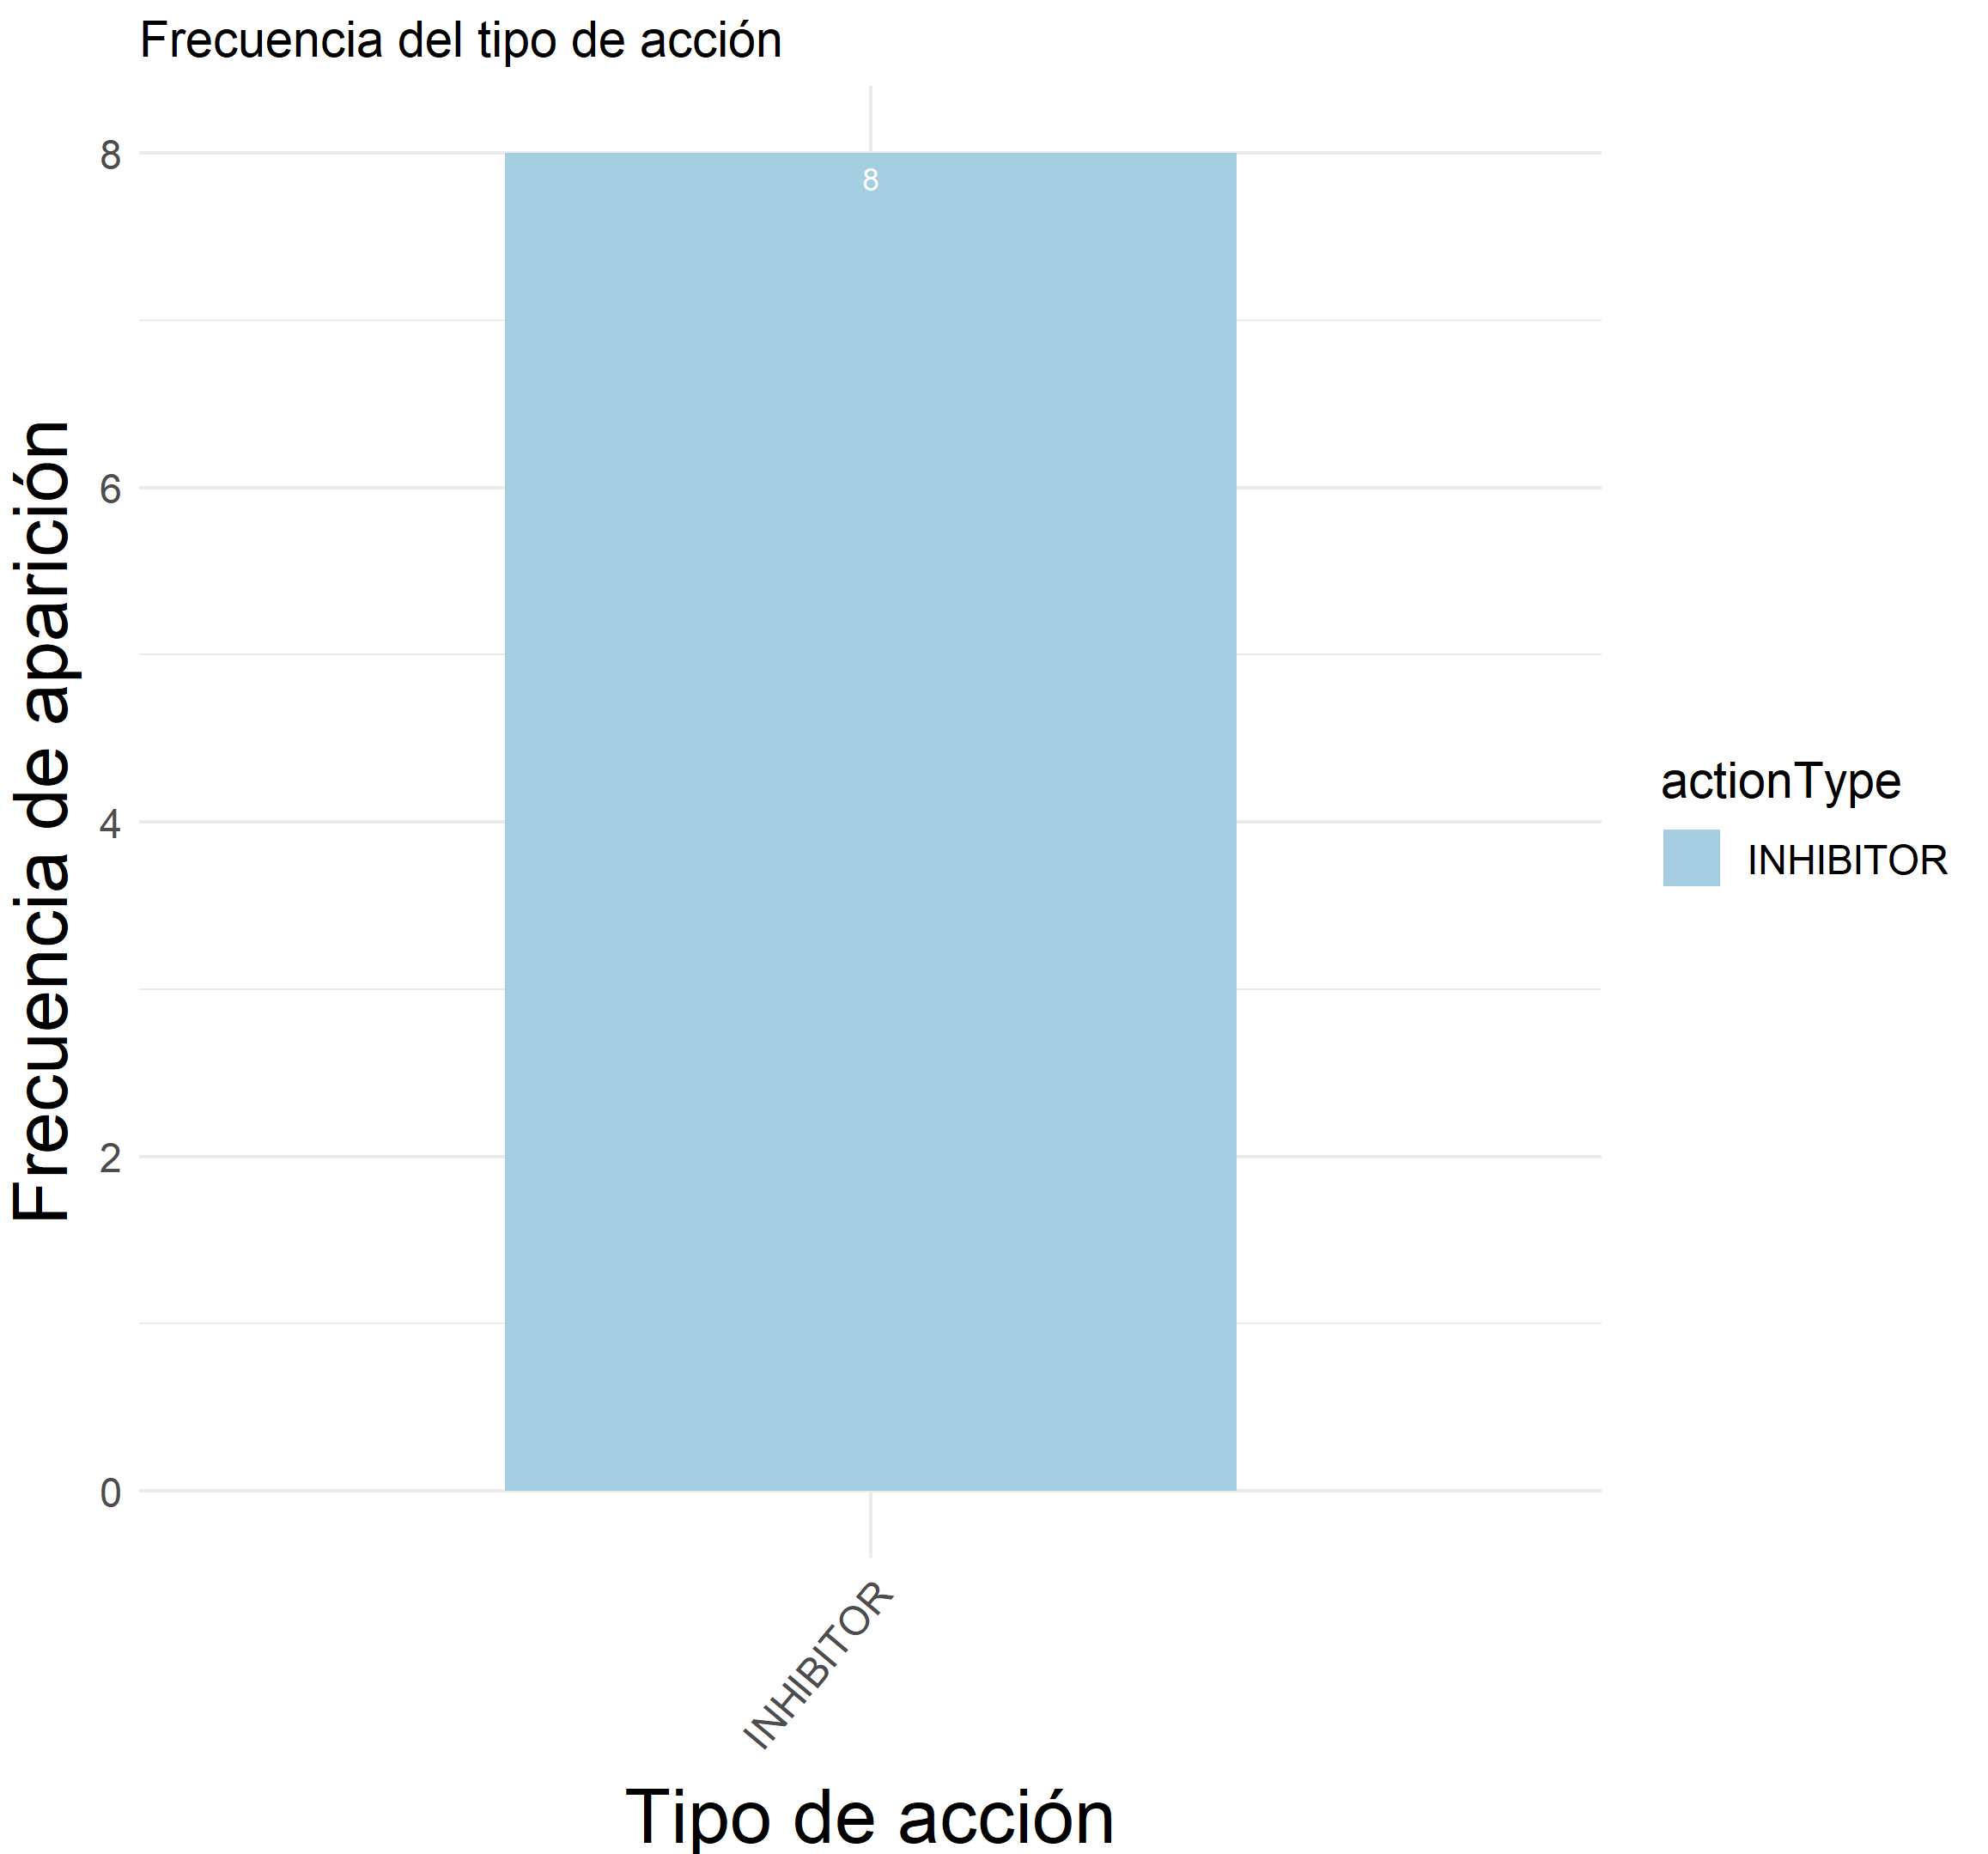
\includegraphics[width=\textwidth]{figures/graficaTipoDeAccion.png}\\
Como se puede comprobar, los inhibidores prevalecen. En el caso de las proteínas de primer grado, veintidós de los treinta y cuatro fármacos encontrados son inhibidores. En el caso de las de segundo grado, la totalidad de los fármacos (ocho) tiene acción inhibidora, significando esto que la mayoría de los fármacos encontrados para estas proteínas se dedican a reducir la actividad de enzimas de manera reversible, acoplándose a ellas.
	
Las siguientes dos gráficas muestran la frecuencia de cada mecanismo de acción existente. Conocer el mecanismo de acción de un fármaco aumenta la información conocida sobre su tipo de acción, pues especifica con mayor profundidad la actividad del fármaco sobre la proteína y la reacción del paciente a él. Con esto podremos ver si algún mecanismo de acción es muy común.

%\clearpage 

\begin{figure}[h!]
			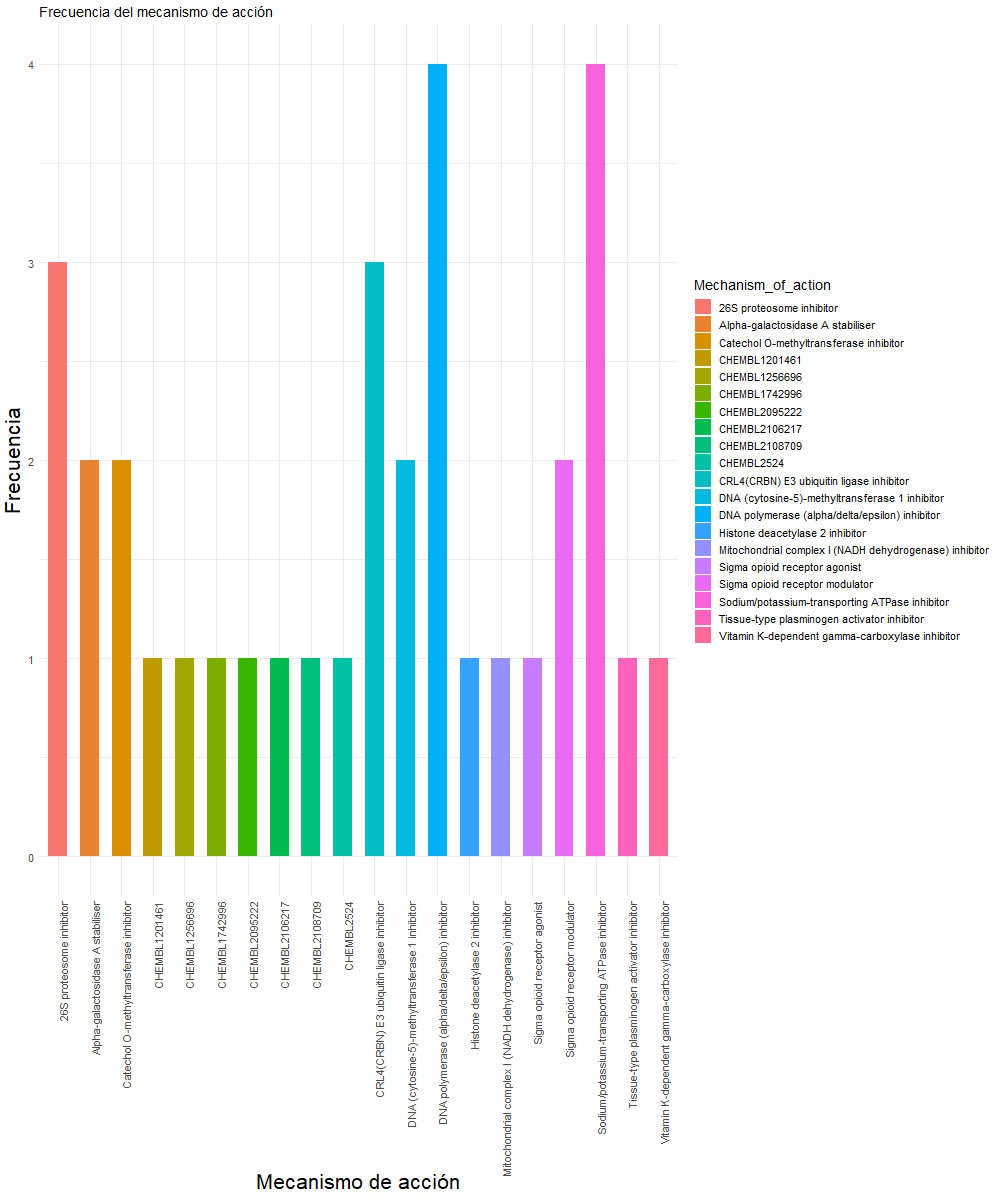
\includegraphics[width=0.9\textwidth]{figures/graficaMecanismoDeAccionProteinas1.png}
			\caption{Mecanismo de Acción, Proteínas de primer grado}
\end{figure}
\clearpage
\begin{figure}[h!]
			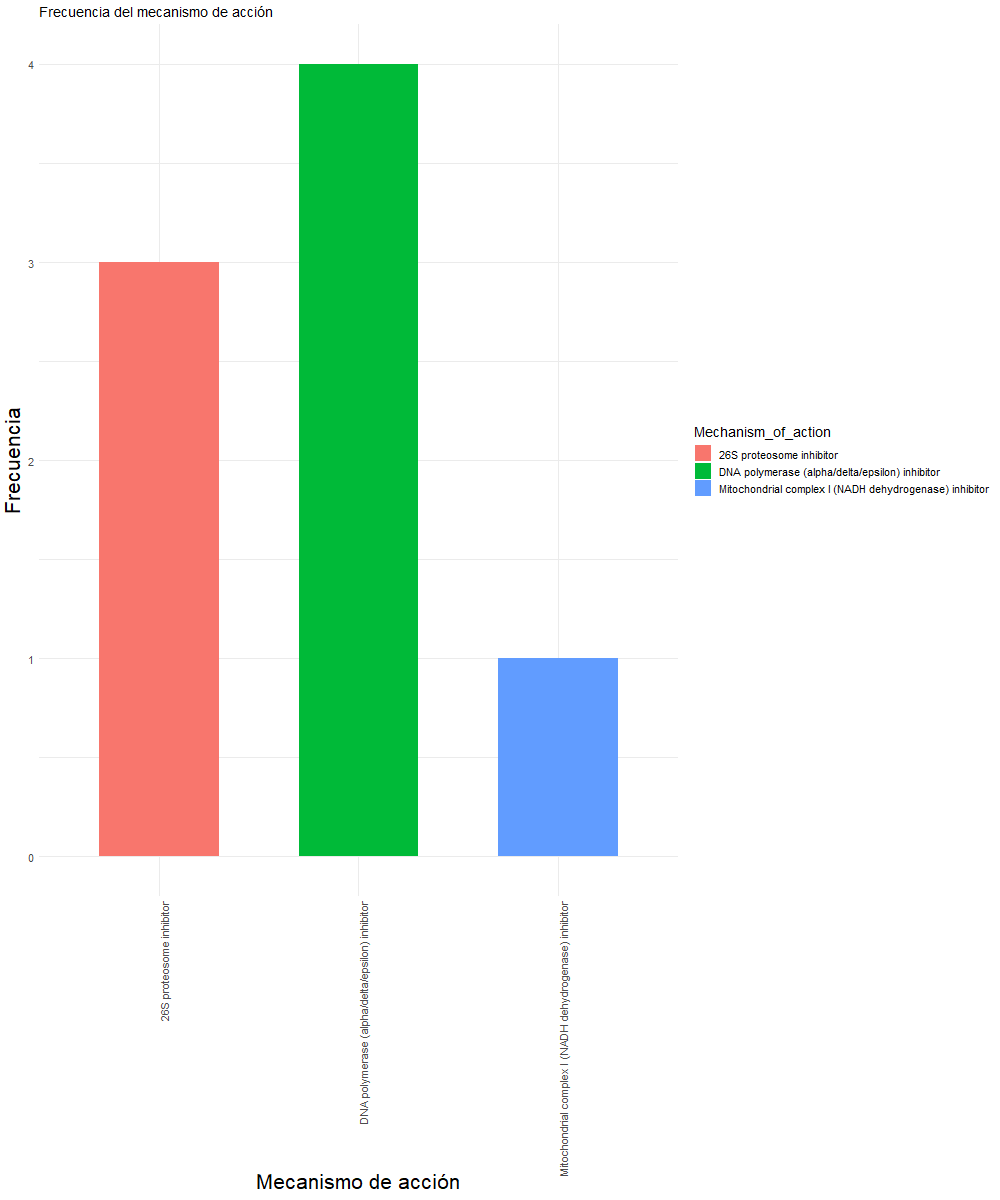
\includegraphics[width=0.9\textwidth]{figures/graficaMecanismoDeAccion.png}
			\caption{Mecanismo de Acción, Proteínas de segundo grado}
\end{figure}

%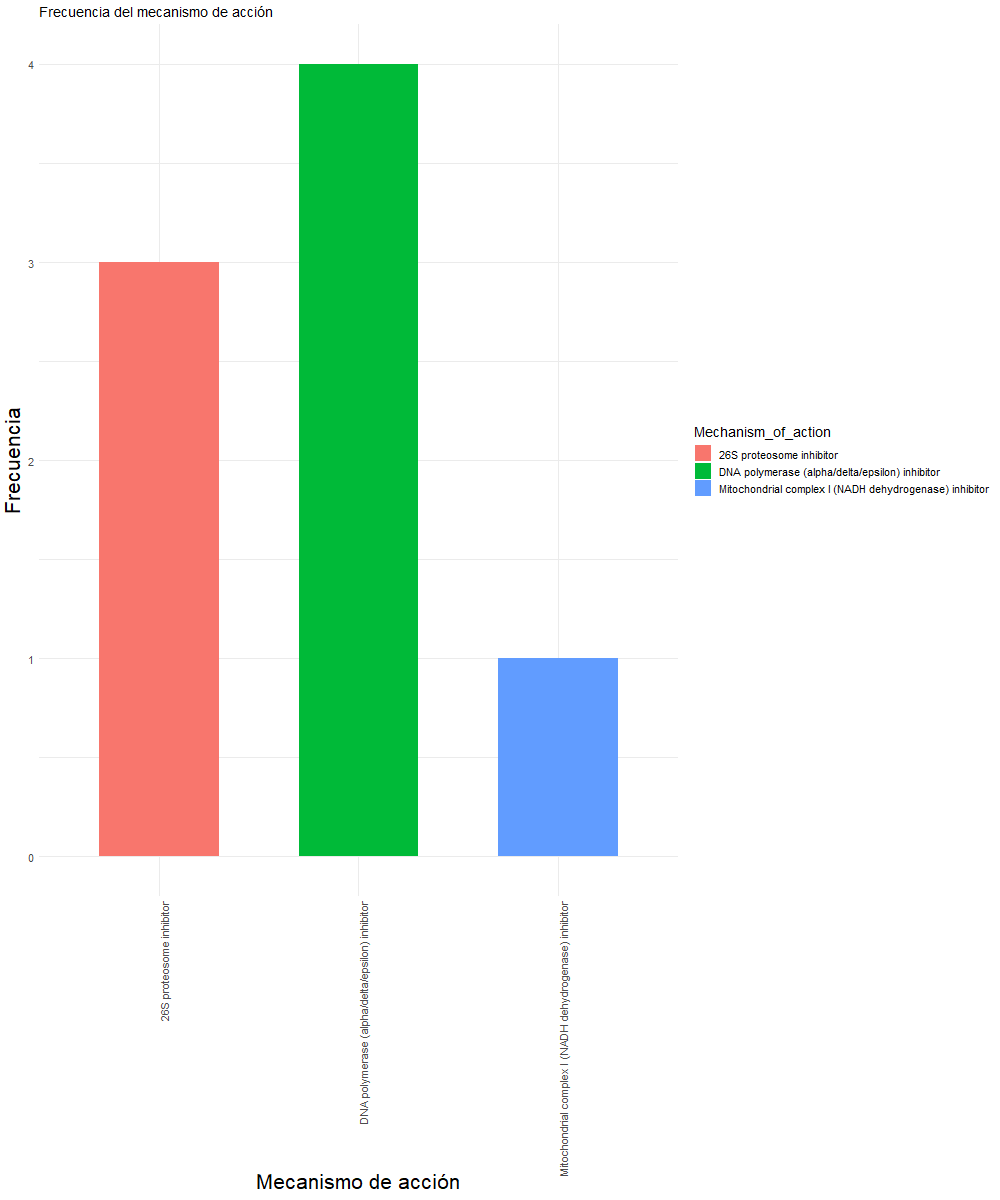
\includegraphics[width=\textwidth]{figures/graficaMecanismoDeAccion.png}\\

%\clearpage 
%\newpage

Observando estas gráficas podemos ver que para las proteínas de primer grado existen cuatro grupos principales de inhibidores, que actúan sobre el proteasoma 26S, la ubiquitina ligasa, la DNA polimerasa y la ATPasa transportadora de sodio y potasio. Otros mecanismos de los que encontramos repeticiones son los estabilizadores de alfa-galactosidasa, inhibidores de metiltransferasa y moduladores de receptor opioide.

En el caso de las proteínas de segundo grado, volvemos a encontrarnos con cuatro fármacos que inhiben a la DNA polimerasa, y tres al proteasoma 26S, además de una que inhibe al complejo mitocondrial. Que se repitan dos mecanismos en ambos tipos de proteínas podría indicar la relevancia de ellos.

Por último, representaremos redes que reflejan la relación entre proteínas y los medicamentos que las afectan. Por tanto podremos encontrar proteínas con mayor cantidad de medicamentos que las puedan afectar.

\begin{figure}[h]
			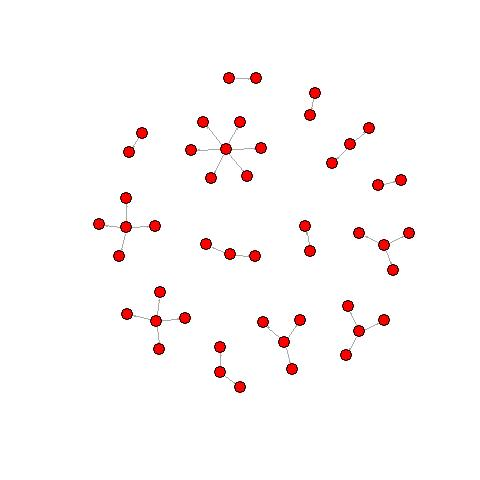
\includegraphics[width=0.9\textwidth]{figures/Red-medicamento-proteina1.jpeg}
			\caption{Interacción proteína-medicamento, Proteínas de primer grado}
\end{figure}
\clearpage
\begin{figure}[h]
			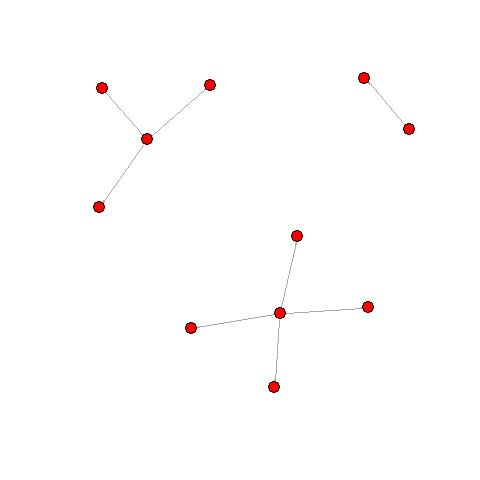
\includegraphics[width=0.9\textwidth]{figures/Red-medicamento-proteina2.jpeg}
			\caption{Interacción proteína-medicamento, Proteínas de segundo grado}
\end{figure}

%\clearpage
A partir de estas redes podemos ver que del primer grupo de proteínas extraemos catorce proteínas relacionadas con nuestros treinta y cuatro fármacos, de las que destaca una con seis medicamentos que la tienen como objetivo.

En el segundo grupo solo se localizan fármacos para tres de las proteínas, pues a dos de ellas las afecta más de un fármaco.

\newpage
		
	\section{Discusión}

Una de las principales apreciaciones de los resultados es que, en ambos caso, el tipo de acción predomintante son los \textbf{inhibidores}, que disminuyen o cesan la acción o creación de otra sustancia.

Por otro lado, podemos ver los mecanimos de acción más presentes:
\begin{enumerate}
\item \textbf{Inhibidor de DNA polimerasa}, fundamentales para la replicación del ADN.
\item \textbf{Inhibidor 26s proteosoma}, un complejo protéico que se encarga de degradar proteínas no necesarias o dañadas.
\item \textbf{Inhibidor de la bomba de Sodio/Potasio}, una enzima que realiza varias funciones en la celula, como mantener el gradiente Sodio/Potasio, el potencial de membrana o de transporte. 
\item \textbf{Inhibidor E3 ubiquitina ligasa}, proteína que recluta una enzima de ubiquitina E2, reconoce un sustrato de proteína y ayuda o cataliza directamente la transferencia de ubiquitina desde el E2 al sustrato de proteína.
\end{enumerate}

Tiene sentido que muchos de nuestros fármacos compartan mecanismo de acción ya que están destinados a grupos de proteínas relacionadas, que comparten función biológica. 

\newpage

	\section{Conclusiones}

El objetivo de esta investigación ha sido encontrar fármacos que puedan combatir el virus SARS-Cov-2 usando la base de datos ChEMBL. Para ello, hemos comenzado nuestro trabajo buscando el interactoma funcional SARS-humano en la literatura científica. Aunque se han realizado numerosos artículos en poco tiempo, aún no se ha descubierto el interactoma funcional completo. Debido a ello, decidimos ampliar la búsqueda de fármacos usando proteínas humanas que interaccionan directamente con las proteínas humanas del interactoma funcional.

Aunque intentamos partir de un conjunto numeroso de proteínas de segundo grado, no ha sido posible debido a que se pierden muchas de ellas al mapear su código de gen al código ChEMBL. Esto se debe a que no existen fármacos en ChEMBL cuyo objetivo sean estas proteínas. Aún así, gracias a las proteínas de segundo grado se consiguen otros ocho fármacos potenciales de fase cuatro. 

Dentro de los fármacos obtenidos, encontramos algunos mecanismos de acción que son más frecuentes que los demás. Como se ha dicho previamente, esto puede deberse a que algunas de las proteínas comparten función biológica. También, pueden tratarse de mecanismos muy estudiados. 

Para futuros trabajos, sería interesante utilizar la información química obtenida de los fármacos potenciales para estudiar el efecto de todos ellos sobre la acción del virus, así como las rutas que siguen en el organismo humano. Además, otra línea de investigación sería estudiar cuál de las proteínas del interactoma funcional es una candidata óptima a desarrollar un fármaco, simulando la repercusión que tendría en el sistema. 

\newpage

	\section{Anexos}

En el siguiente anexo vamos a explicar el significado de cada variable guardada en los archivos csv resultates de la ejecución de nuestro flujo de bash.

\subsubsection{Archivo con información general}

A continuación, se muestran las variables guardadas y su significado:

\begin{itemize}
\item idFarmaco: es el identificador de ChEMBL que tiene el fármaco.
\item idTarget: es el identificador de ChEMBL que tiene la proteína diana del fármaco. 
\item fechaAprovación: fecha en la que el fármaco fue aprobado.
\item canonicalSmile: (Simplified Molecular Input Line Specification o SMILES) es una especificación para describir sin ambigüedades la estructura de una molécula usando cadenas ASCII cortas. 
\item actiónType: indica que tipo acción realiza el fármaco.
\item mechanismOfAction: atributo la forma en la que actúa el fármaco.
\end{itemize}

\subsubsection{Archivo con información química}

A continuación, se muestran las variables guardadas y su significado:

\begin{itemize}
\item AlogP: valor calculado de la lipofilicidad de una molécula expresado como log (coeficiente de partición octtanol / agua).
\item Aromatics\_rings: número de anillos aromáticos.
\item cx\_logd: se define como la relación de concentraciones de todas las especies moleculares (neutras e ionizadas) en octanol dividida por la concentración de todas las especies en medios acuosos al pH especificado.
\item cx\_logp: es el coeficiente de Paritituon octanol/agua calculado utilizando un método basado en fragmentos desarrollado por ACDlabs. 
\item cx\_most\_apka: es el pKa para el grupo más ácido de la molécula.
\item cx\_most\_bpka: es el pKa para el grupo más básico de la molécula.
\item hba: número de aceptores de enlaces de hidrógeno.
\item hba\_lipsinki: número de nitrógenos y oxígenos en la molécula.
\item hbd: número de aceptores de enlaces de hidrógeno.
\item hbd\_lipsinki: número de hidrógenes unidos a átomos de nitrógeno u oxígeno.
\item heavy\_atomos: número de moléculas que no sean hidrógeno en la moléula.
\item molecular\_species: descripción de la especie predominante con pH 7.4. Puede ser ACID, BASE, NEUTRAL o ZWITTERION.
\item mw\_freebase: peso molecular de la forma padre de la molécula.
\item mw\_monoistopic: a masa monoistópica del compuesto calculada como la suma de las masas de los isótopos más abundantes en el compuesto.
\item psa: el área de la superficie polar se calcula mediante el método de P Erti. El cálculo rápido del área de superficie polar molecular es la suma de contribuciones basadas en fragmentos y su aplicación a la predicción de propiedades de transporte de fármacos, Ertl, P., Rohde, B., Selzer, P., J. Medicina. Chem. 2000, 43, 3714-3717.
\item qed\_weight: esta es la estimación cuantitativa de la similitud con las drogas como se describe en: "Cuantificando la belleza química de las drogas” G. Richard Bickerton, Gaia V. Paolini, Jeremy Besnard, Sorel Muresana y Andrew L. Hopkins, Nature Chemistry, 2012, 4, 90-98 Los valores oscilan entre 0-1, donde 1 es el más parecido a una droga y 0 el menos parecido a una droga.
\item ro3\_pass: Regla de 3 pases. Se sugiere que los compuestos que pasan estos criterios tienen más probabilidades de ser aciertos en la selección de fragmentos.
\item rtb: número de enlaces rotativos en la molécula.

\end{itemize}

\newpage
	
	%%%%%%%%%%%%%%%%%%%%%%%%%%%%%%%%%%%%%%%%%%%%%%
	%% OTRA INFORMACIÓN                         %%
	%%%%%%%%%%%%%%%%%%%%%%%%%%%%%%%%%%%%%%%%%%%%%%
	
	\begin{backmatter}
	
		\section*{Disponibilidad de datos y materiales}
			El respositorio de Github usado es: \url{https://github.com/clarajvv/repo\_farm\_COVID}
		
		\section*{Contribución de los autores}
    		L.V.M : Búsqueda de las proteínas del interactoma SARS-Humano, búsqueda de proteínas secundarias en STRING, mapeo de IDCHEMBL, búsqueda inicial de métodos para la extracción de datos de CHEMBL, desarrollo de funciones en R para obtener las relaciones entre proteínas y fármacos y los datos de estos en CHEMBL, creación de gráficas de tipos de acción y mecanismos de acción y guardado de las mismas, escritura anexo, escritura de metodología.
    		
    		C.J.V : Búsqueda inicial de métodos para la extracción de datos de CHEMBL, desarrollo de código en Python para extracción de información desde CHEMBL (fallido), desarrollo en R de pruebas de extracción de relaciones entre proteínas y fármacos y los datos de estos desde CHEMBL, búsqueda de métodos de traducción de IDs de proteínas, ayuda en prueba y error de archivos bash, inclusión de la bibliografía en el informe, comunicación con los profesores, labores de coordinación, maquetación y comentado de las gráficas en el informe,  correcciones finales del informe, escritura de metodología.
    		
    		I.S.J : Documentación sobre el problema \cite{Gysi2020}, búsqueda de métodos de extracción de información de STRING y GO desde R, documentación sobre uso de bash, creación, correcciones y actualizaciones de archivo bash para la instalación de paquetes, creación, correcciones y actualizaciones de archivo de bash para la ejecución del código R, escritura de metodología.
    		
    		P.T.R : Búsqueda de métodos de extracción de información de STRING y GO desde R, recopilación de la bibliografía y creación del archivo para mostrarla, creación de gráficas de interacción y guardado de las mismas, escritura de discusiones y anexo.
    		
		
		%%%%%%%%%%%%%%%%%%%%%%%%%%%%%%%%%%%%%%%%%%%%%%%%%%%%%%%%%%%%%%%%%%%%%%%%%%%%%%%%%%%%%%%%
		%% BIBLIOGRAFIA: no teneis que tocar nada, solo sustituir el archivo bibliography.bib %%
		%% por el que hayais generado vosotros                                                %%
		%%%%%%%%%%%%%%%%%%%%%%%%%%%%%%%%%%%%%%%%%%%%%%%%%%%%%%%%%%%%%%%%%%%%%%%%%%%%%%%%%%%%%%%%
		
		\bibliographystyle{bmc-mathphys} % Style BST file (bmc-mathphys, vancouver, spbasic).
		\bibliography{bibliography}      % Bibliography file (usually '*.bib' )
	
	\end{backmatter}
\end{document}
